\documentclass[../handbook.tex]{subfiles}
\graphicspath{{\subfix{../pics/}}}
\begin{document}

\chapter{A\slash B-тестирование: концепция Fixed Horizon}

В этой главе представлена только методология A/B-тестирования и сопутствующие
ей подводные камни. Конкретные статистические методы можно найти в следующих
главах.

Концепция \emph{fixed horizon} --- база в проведение статистических тестов.
Предполагает, что вы можете запустить эксперимент на определенный промежуток
времени, после которого можно будет подводить итоги. Отвечает на вопросы
сколько должен длиться эксперимент, как сравнивать и интерпретировать
результаты.

\section{Гипотезы}

Когда вы вводите какое-то изменение в своем продукте, а это может быть все что
угодно, вы предполагаете, что что-то изменится. Например, вы решили изменить
интерфейс оплаты, пользователи с большей частотой начнут этим пользоваться; или
вы решили поменять дизайн сайта для того, чтобы к вам пришла новая аудитория,
которой раньше не было. Существенно, есть две вещи:
\begin{enumerate}
    \item фича которую вы хотите реализовать,
    \item метрика на которую повлияет изменение.
\end{enumerate}
Разрабатывая новую фичу, мы \emph{предполагаем}, что когда мы ее внедрим, наша
метрика как-то изменится, например, увеличится. Однако, так ли это на самом
деле?

Может так оказаться, что изменение вообще ни на что не влияет и наша метрика не
поменялась. Это, довольно скептическое отношение к фиче, называется
\emph{основной} гипотезой. Чаще всего в реальном проде именно так и будет
происходить. С другой стороны, наше начальное предположение, что все не зря,
называется \emph{альтернативной} гипотезой.

Помимо здорового скептицизма есть еще одна причина почему основная гипотеза
такая простая --- у нас нет математического аппарата на сложные условия в
основной гипотезе.

\marginpar{
    Альтернативную гипотезу можно формулировать еще и так $H_1: \delta < 0$ или так $H_1: \delta > 0$, это будет зависеть от нюансов задачи.
}
Обозначим через $\delta$ действительное изменение в нашей целевой метрике от внедрения фичи. Тогда основная и альтернативная гипотеза будут записаны так
\begin{equation*}
    \begin{cases}
        H_0: & \delta = 0 \qquad\text{основная гипотеза}\\
        H_1: & \delta \ne 0 \qquad\text{альтернативная гипотеза}
    \end{cases}
\end{equation*}

\marginpar{
    Обратите внимание, что мы ничего существенного не говорим об альтернативной
    гипотезе. \emph{Результатом статистической проверки гипотез является только
    принятие или отвержение основной гипотезы.}
}
Поскольку гипотезы мы проверяем на основе случайных выборок, в них мы врядли
получим хоть когда-нибудь точное равенство $\delta = 0$, даже если бы не
сделали никаких изменений в проде. Так что же мы проверяем на самом деле? Если
бы наша основная гипотеза была верна, то по наблюдаемым значениям мы могли
бы посчитать вероятность обнаружить определенную разницу~$\delta$. Если эта
вероятность окажется маленькой, то у нас уже не будет оснований считать, что
основная гипотеза была верной.


\subsection{Ошибки первого и второго рода.} 
Когда речь идет про нулевую гипотезу мы можем сделать всего две возможные
ошибки:
\begin{margintable}
    % \caption{Ошибки I-го и II-го рода}
    \label{tab:mistakes}
    \begin{center}
        \begin{tabular}[c]{c|c c}
            {\it гипотеза $H_0$} & верна & не верна \\
            \hline
            принята & + & {\it II род} \\
            отвергнута & {\it I род} & + \\
        \end{tabular}
    \end{center}
\end{margintable}
        
\paragraph{Ошибка \emph{первого рода}} --- отклонить нулевую гипотезу, когда
она верна. Вероятность совершения этой ошибки часто обозначают~$\alpha$ и
называют \emph{уровнем значимости}. Ошибку I-го рода обычно фиксируют на уровне
0,05, 0,01 или 0,005, но этот уровень можно менять на любой другой если этого
требует задача.

\paragraph{Ошибка \emph{второго рода}}
\marginpar{
    Критерий проверки гипотезы называется \emph{состоятельным}, если ошибка
    второго рода уменьшается с ростом числа наблюдений.
}
--- принять нулевую гипотезу гипотезу,
когда она не верна. Вероятность совершить ошибку второго рода часто
обозначают~$\beta$, но еще чаще используют $1 - \beta$ называемую
\emph{мощностью} теста. Ошибки II-го рода контролировать сложнее. Для их
уменьшения стараются пользоваться состоятельными критериями.

\subsection{Критерий проверки гипотез}
\marginpar{
    $\mathbf X^a$ --- выборка из контрольного сплита \\
    $\mathbf X^b$ --- выборка из тестового сплита \\
    $\gamma_a = \gamma(\mathbf X^a)$ --- оценка~$\gamma$ на контроле \\
    $\gamma_b = \gamma(\mathbf X^b)$ --- оценка~$\gamma$ на тесте \\
    $d\, = \gamma_b - \gamma_a$ --- оценка эффекта $\delta$.

}
Положим мы хотим оценить параметр~$\gamma$, и мы можем сделать это по какой-то
выборке $\mathbf{X}$. Если нам удастся указать явное распределение~$\mathcal
F_\gamma$ оценок параметра~$\gamma$, то мы сможем вычислить вероятность совершения ошибки I рода.

Положим, что $F_a$ это функция распределения для $\mathcal F_\gamma$ исходя
из выборки~$\mathbf X^a$.

\marginpar{
    \begin{equation}
        p\left(\gamma_l < \tilde\gamma < \gamma_r\right) =
        F_a(\gamma_r) - F_a(\gamma_l)
        \label{eq:accept_hyp_0}
    \end{equation}
}
Проверка гипотезы заключается в том, что мы проверяем, попадает ли наша новая
оценка~$\tilde\gamma$ в интервал $(\gamma_l, \gamma_r)$. Если \emph{да} и
оценка попала в интервал, то мы принимаем нулевую гипотезу, если \emph{нет} ---
отвергаем. Вероятность принять нулевую гипотезу рассчитывается по
формуле~\eqref{eq:accept_hyp_0}. Напомним, что она вычисляется исходя из
предположения, что нулевая гипотеза верна. Так же мы можем вычислить
вероятность совершить ошибку I рода, смотри формулу~\eqref{eq:critical-points} 
\marginpar{
    \begin{equation}
        \alpha = 1 - p(\gamma_l < \tilde\gamma < \gamma_r)
        \label{eq:critical-points}
    \end{equation}
}

Границы интервала называются \emph{критическими точками} и могут быть вычислены таким образом, чтобы вероятность попасть в интервал равнялась $1-\alpha$. Как видно, чтобы найти критические точки нужно уметь брать обратную функцию $F_a^{-1}$, что может быть довольно сложной задачей само по себе. Однако, есть способ проверить гипотезу проще.

\subsection{p-value}
Мы подошли в плотную к понятию \emph{p-value}. Вероятность p-value это
вероятность получить разницу~$d$ которую наблюдаем между оценками теста и
контроля или более худшие варианты. 

При расчете p-value нужно понимать, что значит \emph{хуже}, поэтому конкретная формула зависит от типа альтернативной гипотезы:
\begin{itemize}
    \item $H_1: \delta < 0 \quad \Rightarrow \quad p_v = F_a(\tilde\gamma)$ 
    \item $H_1: \delta > 0 \quad \Rightarrow \quad p_v = 1 - F_a(\tilde\gamma)$ 
    \item $H_1: \delta \ne 0 \quad \Rightarrow \quad p_v = 2\min(F_a(\tilde\gamma),\; 1 - F_a(\tilde\gamma)$ 
\end{itemize}

\begin{marginfigure}
    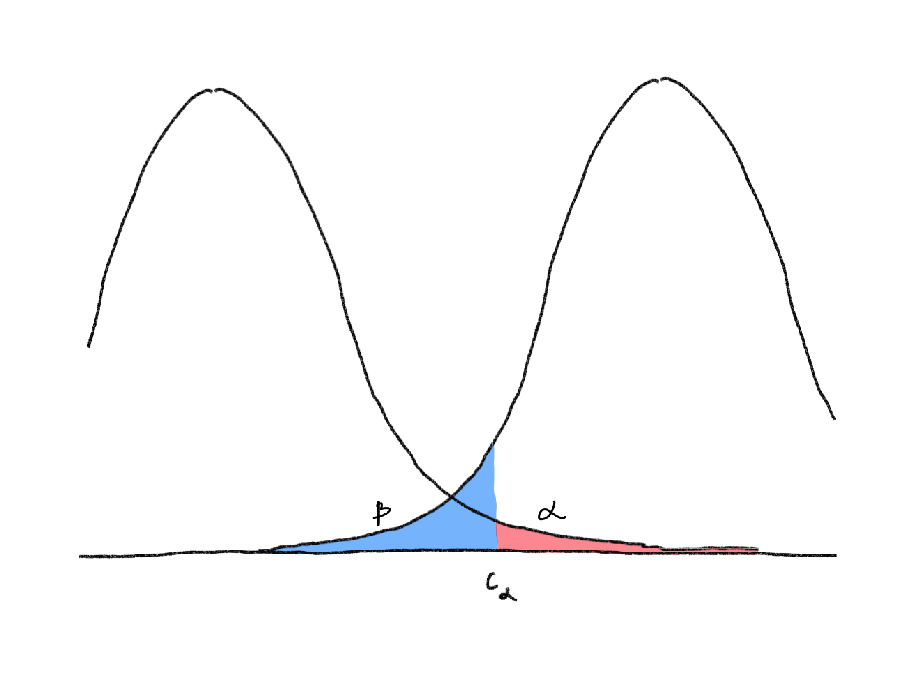
\includegraphics[width=1.1\columnwidth]{critical_points_mistakes_value.pdf}
    \caption{$z_\alpha$ -- критическая точка, $\alpha$ -- вероятность ошибки I рода, $\beta$ -- вероятность ошибки II рода. \\
    Критическая точка не обязана лежать на пересечении плотностей распределений
    двух гипотез. Она определяется только исходя из плотности для нулевой
    гипотезы.
    }
    \label{fig:crit_point}
\end{marginfigure}

Альтернативой к механике проверки гипотез с критической точкой является
проверка гипотез через p-value. P-value вычисляется из предположения, что
нулевая гипотеза верна и определяет вероятность получить такое же значение
критерия или более экстремальное. Нам все равно нужно фиксировать уровень
значимости~$\alpha$ до эксперимента, но не нужно вычислять критическую точку.
Если p-value оказалось меньше~$\alpha$ то нулевая гипотеза должна быть
отвергнута, в противном случае нет оснований отвергать нулевую гипотезу.

В случае если \emph{основная гипотеза верна}, вероятность получить p-value на
определенном уровне имеет равномерное распределение. Например, вероятность
получить p-value из первого дециля равна 10\%, вероятность получить p-value из
второго дециля это $P(\text{p-value} < 0.2) - P(\text{p-value} < 0.1) = 0.1$
тоже 10\% и так далее.

Это показывает, что статистическая проверка гипотез дает
возможность минимизировать ошибку первого рода, но не убирает ее полностью. 

\section{Организация теста}

\marginpar{{\bf Процедура статистического тестирования:}
    \begin{enumerate}
        \item Определить метрику которую проверяем.
        \item Сформулировать нулевую и альтернативную гипотезы.
        \item Зафиксировать уровень стат.значимости~$\alpha$.
        \item Предрасчитать объем необходимой выборки для теста.
        \item Предрасчитать длительность теста.
        \item Запуск теста. В промежуточные результаты не заглядываем.
        \item По истечении времени, интерпретация результатов.
    \end{enumerate}

    % Такая процедура обеспечит, что из всей массы запущенных экспериментов
    % ошибки I рода будут наблюдаться с вероятностью~$\alpha$.
}
Статистическая процедура проверки гипотез позволяет обеспечить вероятность
ошибки I рода на уровне~$\alpha$. Сама процедура не дает гарантий от ошибок, но
позволяет держать их на приемлемо низком уровне. Однако, чтобы процедура
работала необходимо обеспечить дополнительные неявные условия, которые при
рассмотрении чистых статистических критериев часто опускаются.

Итак, предположим, вы уже знаете какую фичу хотите внедрить и определились с
метрикой, которую хотите замерять.

\subsection{Нормальность}
Самые часто применяемые статистические критерии требуют от данных нормальности. Если вы определились с метрикой, то можете попробовать измерить метрику на исторических данных и оценить ее нормальность.

\marginpar{
    $\mu_k$ --- $k$-ый момент \\
    $\sigma$ --- ср.кв.отклонение
}
Проверять данные на нормальность стоит не слишком тщательно. Данным достаточно только \emph{напоминать} нормальные, чтобы использовать большинство критериев в которых подразумевается, что данные нормальные. Если подходить к проверкам строго, то ничто и никогда невозможно будет проверить. 

Точно необходимо проверить:
\begin{enumerate}
    \item \emph{Выбросы.} Отсутствие выбросов достаточно критичное условие. Если в данных есть выбросы, то их нельзя считать нормальными. С другой стороны если эти выбросы убрать, возможно уже можно будет работать.

    
    \item \emph{Асимметрия.}\marginnote{ \[A = \frac{\mu_3}{\sigma^3}\]}
        Нормальные данные должны быть симметричными, поэтому если наблюдается асимметрия, то данные не нормальные. Возможно сможет помочь логарифмирование. 

    \item \emph{Эксцесс (kurtosis)} --- отклонение от колоколообразности.
        \marginnote{ \[\gamma_2 = \frac{\mu_4}{\sigma^4} - 3\]}
        Пограничным случаем колоколообразности можно считать равномерное распределение, а вот бимодальность гистограммы уже явный признак, что данные не нормальны. Еще чем больше наблюдений в данных, тем все-таки ближе должна быть гистограмма к нормальному распределению. За критерий можно взять выборку в $n=150$, чей график должен быть похож на колокол.
\end{enumerate}

Если в выборке менее 2000 объектов, то применяется метод Шапиро-Уилка, если же объектов больше, то используется критерий согласия Колмогорова-Смирнова.

Возможно ваши данные не подчиняются нормальному закону распределения. В этом случае можно попробовать удалить из данных выбросы или преобразовать таким образом, чтобы данные стали нормальными. Возможно, даже и то и другое.

% \subsection{Удаление выбросов}
\paragraph{Преобразование Бокса-Кокса.} 
\marginpar{
    \begin{equation}
        \label{eq:box-cox}
        x_{i,\lambda} = 
        \begin{cases}
            \frac{x_i^\lambda - 1}{\lambda} & \text{если } \lambda \ne 0, \\
            \log(x_i) & \text{если } \lambda = 0.
        \end{cases}
    \end{equation}
}
это преобразование исходного набора
данных. Применяют в основном с целью устранения выбросов. Например,
при~$\lambda = 0$ это обычное логарифмическое преобразование.
Параметр~$\lambda$ подбирается методом оптимизации правдоподобия.

{\it Почему такая формула?} Логарифмическое преобразование хорошо себя
зарекомендовало, но оно не всегда справляется. Замечено, что $(\log x)' =
1/x$. Преобразование Бокса-Кокса это обобщение до функций чьи производные
равны $1/x^\lambda$.

\paragraph{Расстояние Махалонобиса.}
\marginpar{
    $m$ --- выборочный вектор мат.ожидания \\
    $S$ --- выборочная матрица ковариации
}
\begin{marginfigure}
    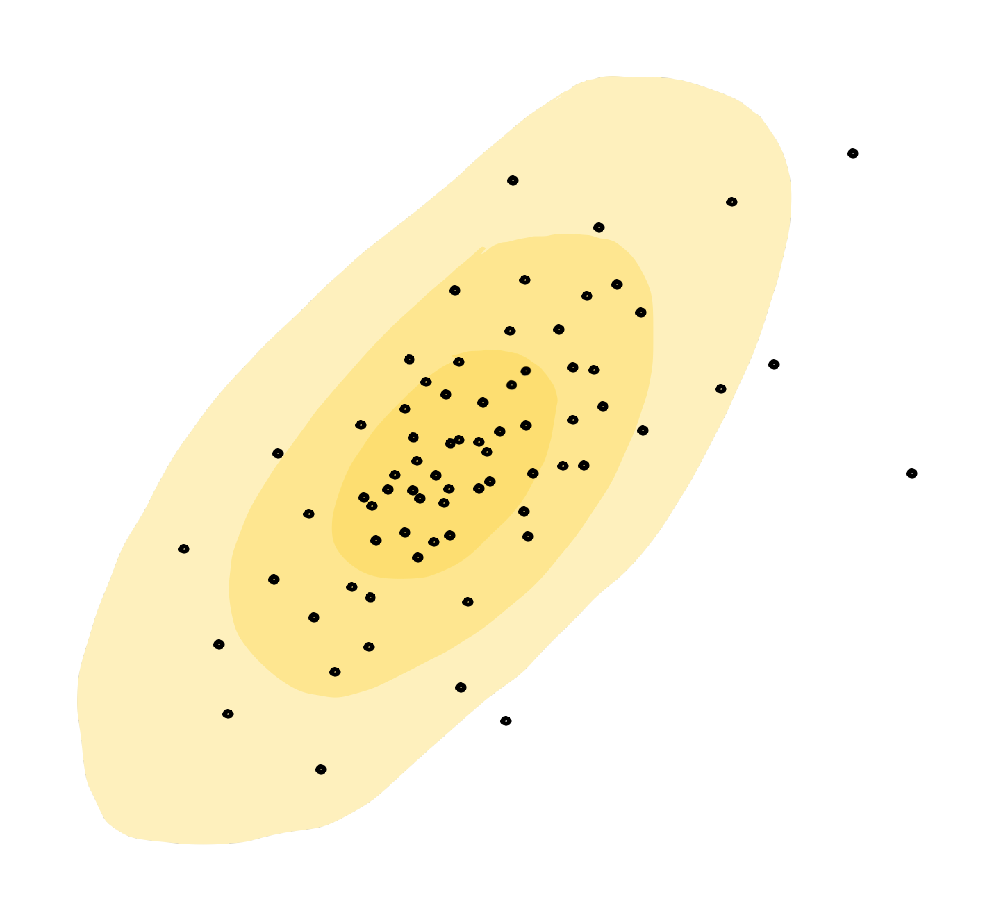
\includegraphics[width=0.8\columnwidth]{mahalanobis.pdf}
    % \caption{выбросы через расстояние Махаланобиса}
    % \label{fig:mahalanobis}
\end{marginfigure}
Для многомерных данных можно предположить, что они распределены по какому-то многомерному нормальному закону распределения. Если центр (мат.ожидание) и матрицу ковариации для датасета, то можно определить расстояние Махалонобиса. Так мы получим аналог много\-мерной дисперсии и сможем вычислить отклонение от среднего
\begin{equation}
    \label{eq:mahalanobis}
    d = \sqrt{ (x - m) S^{-1}(x-m)^T}
\end{equation}
Мы можем использовать это расстояния для определения 95\% границы (или любой другой) чтобы построить область допустимых значений. Сэмплы за вычисленной границей будут считаться аутлайерами. Поскольку вычисление границы может оказаться дорогим, можно провести упрощенное действие: рассчитать для каждого сэмпла расстояние~\ref{eq:mahalanobis} и отрезать 5\% граничных квантилей.

% \subsection{Бакетный тест}
\paragraph{Бакетный тест.}

\marginpar{
    $K = 30$ обычно достаточно, чтобы грубо оценить мат.ожидание
}
Если удаление выбросов не помогает сделать данные нормальными, например, есть выраженная асимметрия, то можно воспользоваться \emph{бакетным тестом}. Для этого разделим выборку на непересекающиеся подвыборки по $K$ элементов и измерим в каждой из них мат.ожидание. Так мы получим распределение оценок мат.ожидания, которое должно подчиняться центральной предельной теореме. Естественно, это все будет работать только если изначально у нас была большая выборка данных, поэтому рекомендуется использовать бакетный тест если объем выборки $N \geq 3000$.

\subsection{A/A-тестирование}
A\slash A-тесты те же самые A\slash B-тесты, но на исторических данных.
Зачастую их проводят с целью провалидировать какие-то предположения перед
запуском теста. Может оказаться так, что какие-то критерии не работают потому,
что нарушаются условия (каким-то неизвестным нам образом) применения этих
критериев. В этом случае A/A-тесты не сойдутся и это повод выяснить причины и
устранить их до запуска полноценного A/B-теста.

\paragraph{Ошибка сплитования.}
\marginpar{
    Может так случиться, что есть большая текучка пользователей и пользователи предпериода почти не совпадают с теми пользователями которые будут в тесте. Тогда такая проверка будет невалидной.
}
Допустим мы ввели новую процедуру сплитования для A/B-эксперимента и хотим проверить сплиты на однородность. Запустим наш эксперимент который планировали, но на исторических данных (предпериод). Поскольку мы считаем эксперимент в прошлое, когда у нас еще не было фичи которую только собираемся раскатить, оба сплита должны вести себя одинаково. То есть должна победить гипотеза~$H_0$ о равенстве метрик.

\paragraph{Проверка стат.критерия.}
\marginpar{
    Самый частый способ разбить на выборку на две части, это отправить четные
    элементы в тест, а нечетные в контроль (или наоборот). Поскольку такой
    способ дает только одно возможное разбиение перед разбиением добавляют
    хэш-функцию и к ней соль, что дает возможность сделать много случайных
    разбиений.
}
Допустим, мы сконструировали некоторый
стат.тест и хотим проверить хорошо ли он работает. В этом случае тоже могут
помочь A\slash A-тесты. Процедура такая:
\begin{marginfigure}
    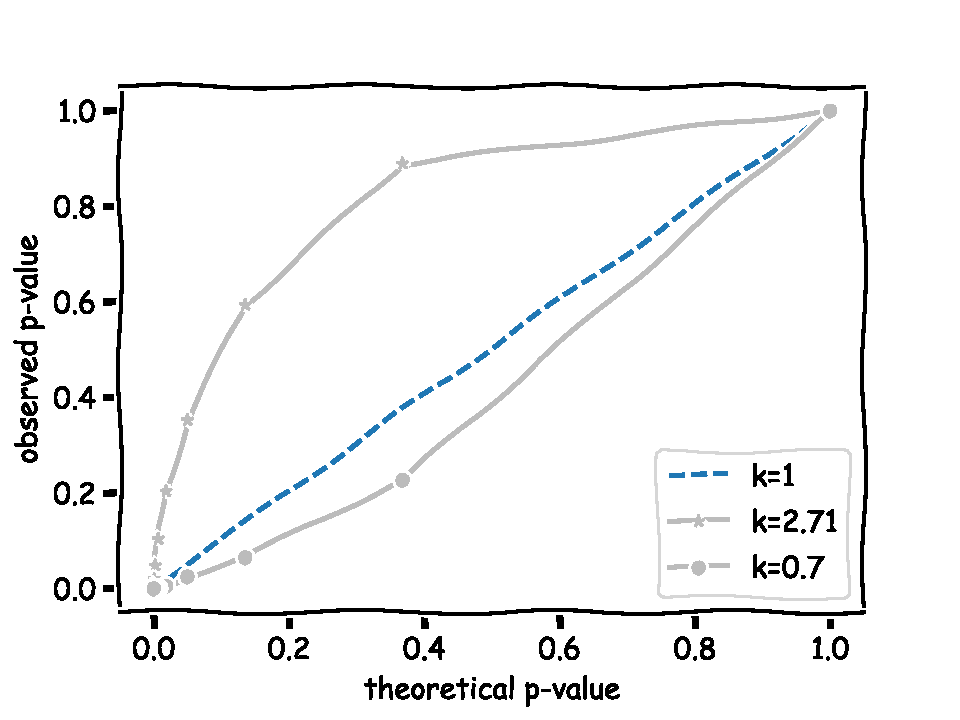
\includegraphics[width=1.1\columnwidth]{theoretical_observed_p_value.pdf}
    \caption{Пример оценки критерия. В случае если критерий корректен, мы
        должны получить диагональную линию. \\
        Данные случайным образом генерируются из экспоненциального
        распределения. В качестве критериев проверки подбираются
        гамма-распределения с различными~$k$. То есть действительно, проверка
        показала, что лучше использовать экспоненциальный критерий.
    }
\end{marginfigure}
\begin{enumerate}
    \item Сделаем 1000 разбиений выборки предпериода различными солями.
    \item На каждой выборке проведем эксперимент и посчитаем значение~$p_{value}$.
    \item Построим гистограмму полученных~$p_{value}$.
    \item Если гистограмма получилось не равномерной, то выбранный критерий не работает и в нашем тесте есть систематическая ошибка. 
\end{enumerate}

Если на гистограмме построенных $p_{value}$ нет равномерности, то у нас нет
гарантии, что $p_{value} < \alpha$ действительно будет встречаться в $\alpha\%$
случаев.

\subsection{Эффективность и длительность}

\paragraph{Minimum Detectable Effect} \emph{(MDE)}
\marginpar{
    $\delta$ --- minimum detectable effect
    \begin{equation}
        \label{eq:mde_simple}
        \delta = (z_{1 - \alpha/2} + z_{1 - \beta})
            \sqrt{ \frac{4\cdot s_h^2}{n_h}}
    \end{equation}
    $s_h$, $n_h$ --- исторические ср.квадратическое и общий объем выборки (аудитории)
}
-- минимальное изменение
которые мы сможем зафиксировать во время эксперимента. Зачем вообще считать
MDE? Допустим мы знаем какой минимальный эффект нам нужно обеспечить чтобы
оправдать затраты на эксперимент. Тогда исходя из этого знания, мы можем
посчитать необходимый объем выборки, при которой достигается желаемый MDE. 

\marginpar{
Снизить такой MDE можно тремя способами:
\begin{enumerate}
    \setlength\itemsep{0em}
    \item Увеличить объем выборки~$n_h$
    \item Снизить дисперсию~$s_h$
    \item Снизить мощность $1-\beta$
\end{enumerate}
}
В простейшем случае для рассчета MDE можно пользоваться
формулой~\eqref{eq:mde_simple}, но с ней тоже нужно быть аккуратным потому, что
она верна только для нормального распределения. Подробности о том как выводится
формула в пункте~\ref{sec:sample_value}. 

%# Из формулы~\eqref{eq:mde_simple} можно сделать вывод, если необходимо обеспечить низкий MDE то сделать это можно тремя способами:
%# \begin{itemize}
%#     \item Увеличить объем выборки~$n_h$,
%#     \item Снизить дисперсию~$s_h$,
%#     \item Снизить мощность $1-\beta$.
%# \end{itemize}


\paragraph{Длительность эксперимента}
зависит от необходимого объема выборки,
однако, необходимо учесть еще и сезонность. Если не учесть сезонность, то это
получится, что в выборке могут быть не соблюдены пропорции из генеральной
совокупности и числа могут быть не корректные. Например, есть дневная
сезонность, мы запустили эксперимент в полночь и к 6 утра уже добили нужные
объемы. Однако активность пользователей ночью отличается от активности
пользователей днем. В итоге мы получим либо смазанные результаты, либо
некорректные. Поэтому расчетную длительность округляют до кратности сезонности.

С другой стороны можно поступить проще. Поскольку сезонность известна, известны  объемы пользователей, мы можем выбрать несколько длительностей и посчитать ожидаемые MDE при разных длительностях и выбрать подходящий.

\section{Результаты теста}

Важно выдержать корректную процедуру тестирования и интерпретации результатов.
Даже если окажется, что на тесте показатель выше это еще не означает что тест
успешный или провальный.

\subsection{Ошибка подглядывания}
Ошибка подглядывания возникает когда мы заглядываем в результаты теста до
окончания самого теста (в промежуточное время). В этот момент человек может
увидеть промежуточный результат p-value~$< \alpha$. Во время подглядывания
может возникнуть соблазн дождаться когда p-value упадет ниже уровня
стат.значимости и остановить эксперимент. На самом деле график p-value в
процессе эксперимента может несколько раз опускаться ниже стат.значимости. Это
будет происходить случайно.\sidenote{\fullcite{karpov:ab_peeping}}

Если же следить за p-value пока он не опустится ниже~$\alpha$ мы увеличим вероятность ошибки I рода и перестанем ее контролировать. И по сути будем выдавать желаемое за действительное.

\subsection{Sample ratio mismatch (SRM)}

\emph{Sample ratio mismatch} --- это несоответствие отношений между тестовой
выборкой и контролем на тесте и в ожиданиях.

\marginpar{
    Критерий хи-квадрат очень чувствительный и может помечать даже самые слабые
    несоответствия как значимые, поэтому для теста используют низкий порог
    стат.значимости $\alpha = 0.01$ или даже $\alpha=0.001$.
}
Например, мы хотели набрать по 50 тысяч пользователей в каждом сплите за время
эксперимента, а получили 47 и 50 тысяч. Разница может оказаться не
существенной, а может и сильно исказить результаты. Если в ``непришедших'' 3
тысячах посетителей были нелояльные пользователи, то у нас изменились пропорции
между пользователями на контроле и в тесте. Значит и результаты будут
некорректными.

% TODO: надо узнать этот критерий
Для проверки SRM используют критерий хи-квадрат.

\subsection{Доверительные интервалы}
\marginpar{
    $\delta$ --- оценка эффекта от эксперимента \\
    $\alpha$ --- уровень стат.значимости
}
На этапе расчета теста нам важно, чтобы итоговый прирост~$\delta$ был выше
порога MDE, то есть $\delta > MDE$. Когда мы проводим вычисление результата мы на самом деле проводим
вычисление эффекта по выборке, то есть в реальности числа могут отличаться.
Чтобы быть уверенными в своих результатах можно построить доверительный
интервал на оценку прироста. Реальный эффект будет лежать в доверительном интервале с вероятностью $1 - \alpha$.

\paragraph{Красный тест.}
\begin{marginfigure}
    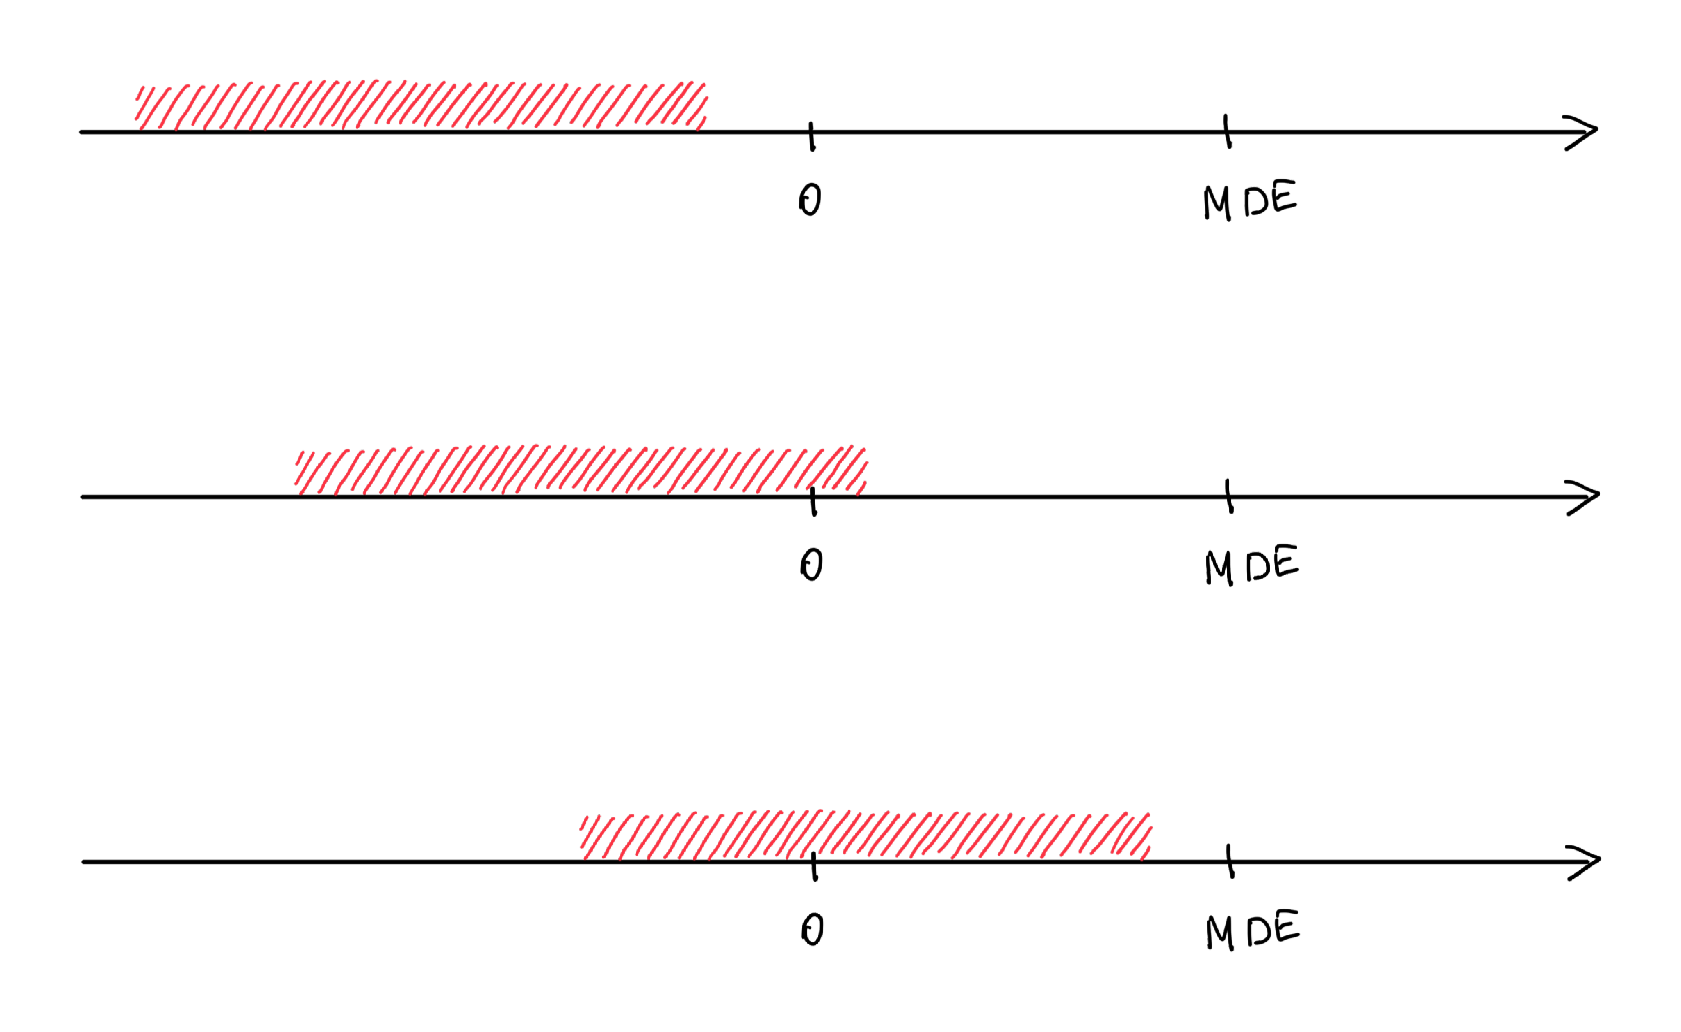
\includegraphics[width=1.1\columnwidth]{ab-test-red.pdf}
    % \caption{Красный тест}
    % \label{fig:move_y}
\end{marginfigure}
Допустим мы построили доверительный интервал для оценки~$\delta$ и он лежит
полностью правее нуля, то есть эффект от эксперимента отрицательный. Мы не
добились желаемого эффекта и значит от фичи стоит отказаться.

Аналогично, если интервал покрывает ноль, но не затрагивает MDE. Получается мы
не видим стат.значимого отклонения от нуля, зато видим стат.значимое отклонение
от MDE. Фичу не стоит раскатывать.

\paragraph{Серый тест.}
\begin{marginfigure}
    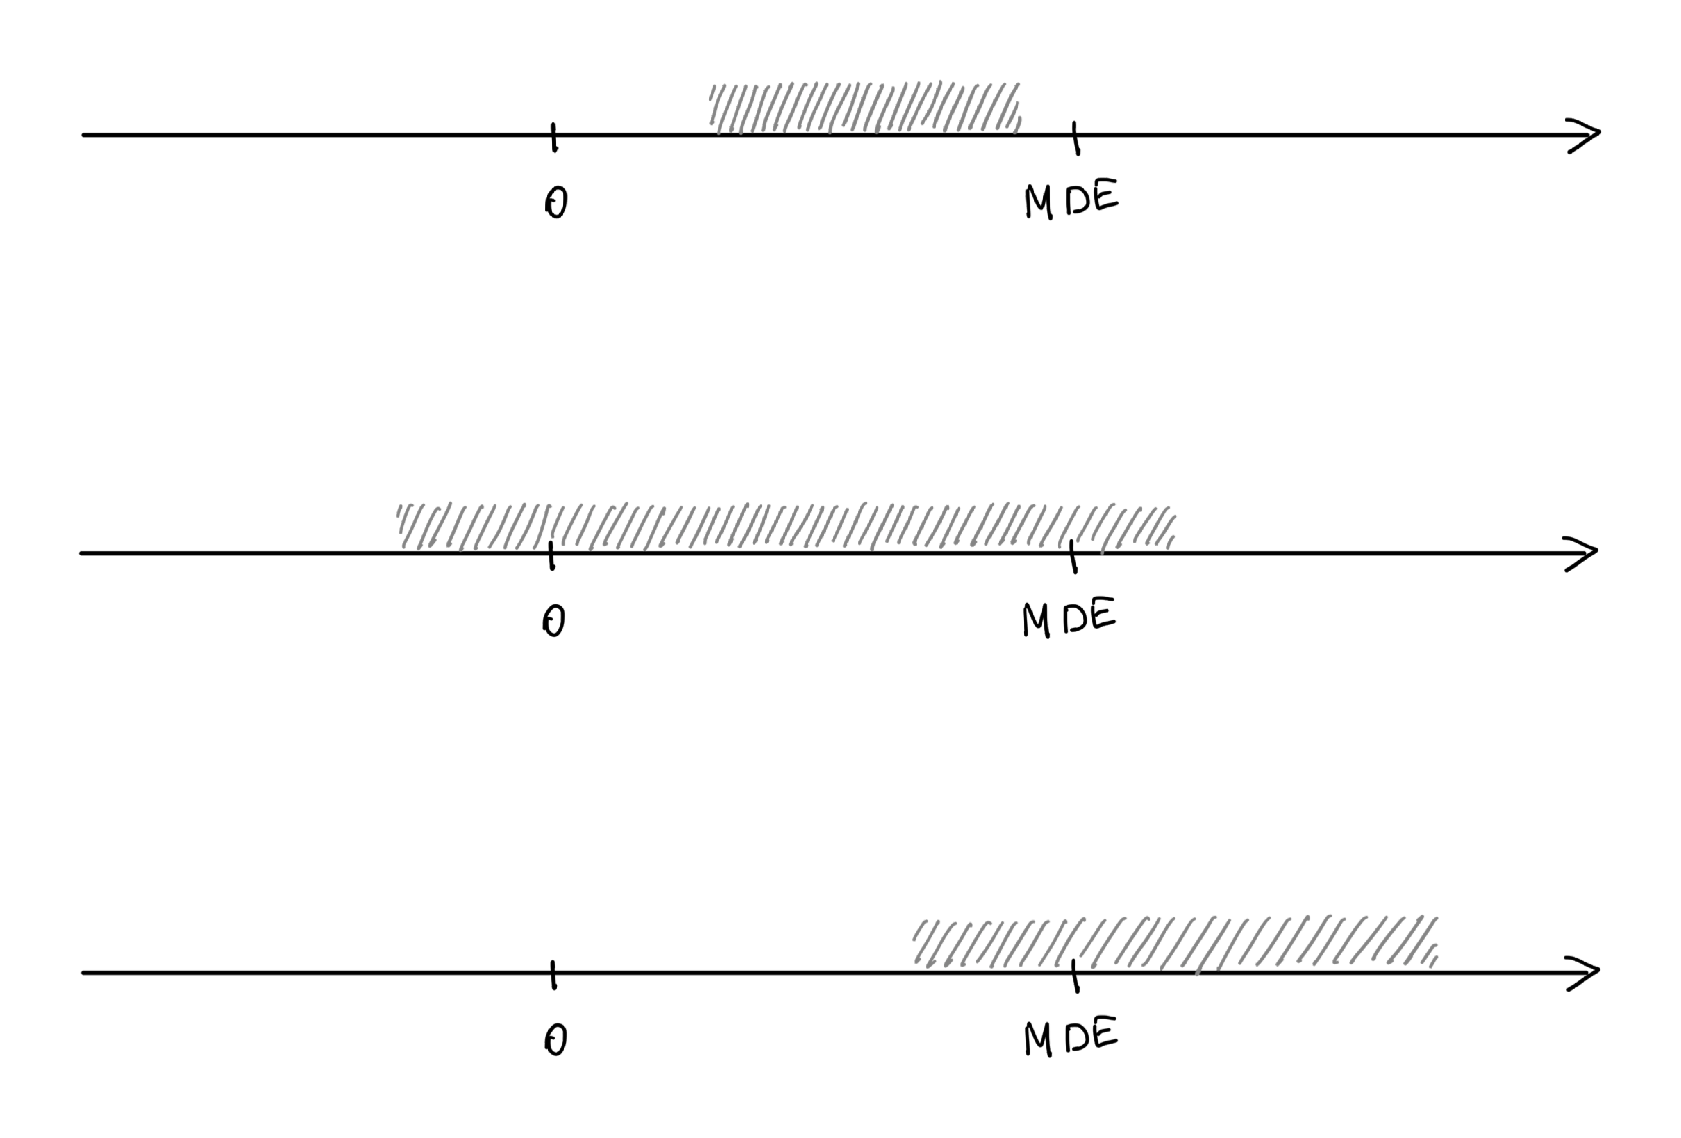
\includegraphics[width=1.1\columnwidth]{ab-test-gray.pdf}
    % \caption{Серый тест}
    % \label{fig:move_y}
\end{marginfigure}
Если доверительный интервал покрывает и 0 и MDE, это означает, что нет
стат.значимых отличий ни от нуля, ни от MDE. Видимо для теста нужно больше
времени. Здесь нужно смотреть по ресурсам, продление А/B-теста может
заблокировать другие эксперименты, а эффекта мы можем и не получить.

Возможна еще одна ситуация, когда у нас есть стат.значимые отличия и он нуля и
от MDE, но эффект который мы получили меньше, $0 < \delta < MDE$. В этом случае
тоже решение принимать стоит по обстоятельствам, эффект положительный, но ниже
наших затрат.

В случае если доверительный интервал покрывает MDE, но не покрывает ноля, мы
можем утверждать, что эффект положительный, но нет гарантий, что он превосходит
MDE, поэтому эксперимент стоит продлить, чтобы сделать более точную оценку
эффекта. Доверительный интервал должен сузиться на большем объеме данных и
возможно уже не будет покрывать MDE и сможем сделать более уверенные выводы.

\paragraph{Зеленый тест.}
\begin{marginfigure}
    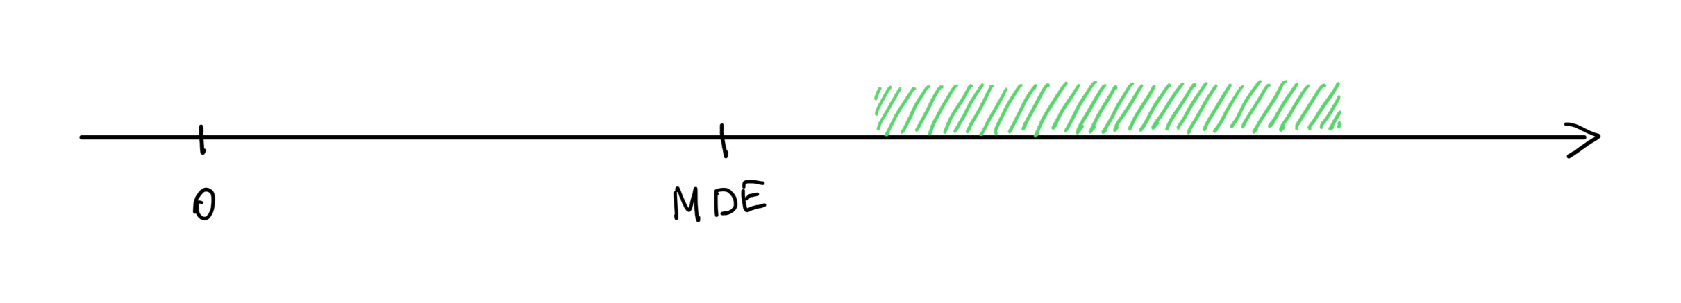
\includegraphics[width=1.1\columnwidth]{ab-test-green.pdf}
    % \caption{Зеленый тест}
    % \label{fig:move_y}
\end{marginfigure}
Если доворительный интервал полностью лежит правее MDE, значит мы достигла стат.значимого результата тест, можно принимать. Реальный эффект от внедрения фичи будет выше MDE.


\end{document}
